

\documentclass[12pt,a4paper]{book}


\input{Files/Packages}

\input{Files/Macros}


\title{Game Programming with SDL}
\author{Ranim Tom}
%\date{August 2021}


%******** Abbreviations **********

% to change the name of Nomenclature to list of abbreviation
\renewcommand{\nomname}{List of Abbreviations}

% for list of abbreviations and acronyms
\makenomenclature



\begin{document}

% downloaded template: Cover of the Report
%\input{content/title_page_1} 


\maketitle

\tableofcontents


% to make the list of abbreviations and acronyms appear 
% in first pages of the report
\printnomenclature


% to make the todo list appear as a table of content
\listoftodos

% To adjust the header in the report/book

\pagestyle{fancy}
\fancyhf{} % Clear header and footer
\rhead{\rightmark}
\lhead{Chapter \thechapter}
\rfoot{Page \thepage}





\chapter{Game Development with C++ and Lua}

\section{Introduction}

In this chapter, we build a simple 2D game but nevertheless functional game with \verb|C++|. We will go in this section about the outcomes and the deliverable of this project.\\

\begin{enumerate}

\item \underline{Game Engine Architecture:}

We discuss programming pattern used inside a game engine. So it's not about making games only (like drawing some \verb|png| structures and making them move), no it's about an application called game engine at $\mathrm{1}^\mathrm{st}$, then using this engine to make many game.


\item \underline{Creating a final game:}

To fix the concepts and the idea and to understand more, we will also create a game using (where we have all the idea of attack,collision, motion,$\cdots$) this engine. Also, we will use \verb|Lua| (a programming scripting language) to enable the users and the level designers to change some of the behavior of the game. An example is shown \autoref{fig:first_game_engine_cpp:product_game_and_lua}, where the \verb|Lua| file is used to set some parameters of the game

\newpage
\begin{figure}[h]
\centering
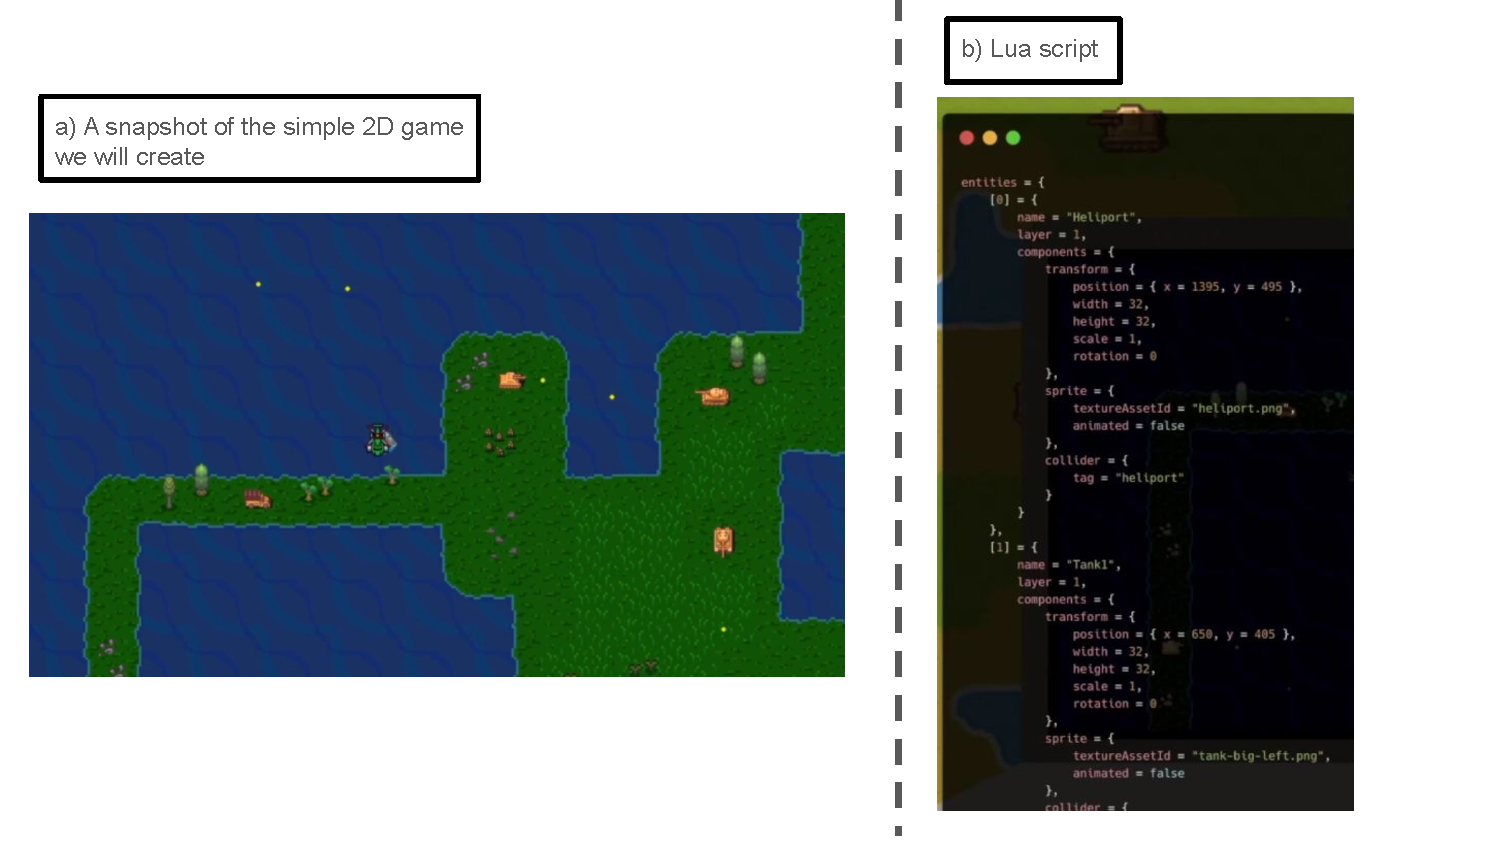
\includegraphics[scale=0.6,frame]{Figures/first_game_engine_cpp/product_game_and_lua}
\caption{Goal of this project in this chapter}
\label{fig:first_game_engine_cpp:product_game_and_lua}
\end{figure}


\item \underline{Use modern C++ and other helper libraries:}

We will learn throughout the course the use of modern \verb|C++| (like templates,smart pointers,$\cdots$).

Also we will use some other \tbi{helper libraries}: \verb|SDL| for graphics,audio,$\cdots$, \verb|ImGui| to create application, \verb|glm| for math manipulation (such as matrix operation,$\cdots$), and finally \verb|Lua|.

\item \todo{Outcomes and deliverable} \underline{\textit{Outcomes and deliverable}:} \textit{to repeat later the intro from the implementation point, and write down  the role of each concept.} 

\end{enumerate}


\newpage
\section{Installation and Configuration}

Now in this section we will see how to install and configure the necessary libraries, dependencies, and make sure that everything run well.

\subsection{C/C++}

See \ref{Intro:sub:setting_C_and_SDL_in_Linux}.

\subsection{SDL Installation}

\begin{itemize}

\item \verb|sudo apt install libsdl2-dev|

    \begin{itemize}
        \item This is the core of the \verb|SDL| library.
    \end{itemize}

\end{itemize}

But this is not enough, we need also some \tbi{extensions}

\begin{itemize}

\item \verb|sudo apt install libsdl2-image-dev| (to load \verb|png| images,$\cdots$)

\item \verb|sudo apt install libsdl2-ttf-dev| (work with fonts)

\item \verb|sudo apt install libsdl2-mixer-dev| (for sounds)

\end{itemize}

\subsection{Lua}

\verb|sudo apt install liblua5.3-dev|

\subsection{Command Exploring directory structure}

A nice command to explore the structure of some project, we can use \verb|tree -d|, and it will give the hierarchy of our folder in a tree structure, with all the directory in it.

\section{Building}

Now once we install things, we need to test if our installation is correct. We will use makfile to automate our compilation, linking and running process.

\subsection{Makefile}

\verb|Makefile| are files processed (read) by a tool named \verb|make|, which is given from \verb|gnu| community (and directly installed when we ran \verb|build-essential|).\\


When defining rule with \verb|Makefile|, it is necessary to indent the rule with a tab.


\newpage
\section{Compiling and testing all dependencies}

Till now, we compiled and verified that \verb|C++| and \verb|SDL| (along with extensions) are compiled correctly.

However, we need also to test and see the compilation for the $\mathrm{3}^\mathrm{rd}$ party libraries installed inside the \verb|lib| folder in our project. 

Unlike \verb|SDL|, which is installed \tbi{globally in our linux system}, the libraries in \verb|lib| folder are installed \tbi{locally inside our project}, so we need to instruct the compiler to search inside the \verb|lib| folder, to find the necessary header files.

\subsection{sol and lua libraries}

For \verb|sol| library, we added also extra linker flags in order to have the compiler to link between \verb|ol| \verb|lua|

\subsection{Binary Libraries}

When we asked the package manager (\verb|apt|) to install \verb|SDL| and \verb|lua|, it will install \tbi{binary version} of these libraries suitable for our OS (in my case \verb|Linux|). So every time we run \verb|make build|, we don't compile all the source code of \verb|SDL| and \verb|lua|, we only compile our source code, then when reaching the liking stage, the linker fetch the binary of these libraries.

This will save a huge compile time, because compilation time can be headache in \verb|C/Cpp|.

\subsection{Static and Dynamic Libraries}

One final topic that might be useful to discuss is the difference between \verb|.lib| and \verb|.dll| files.\\

This small article is mostly for curiosity purposes so we understand what programmers are talking about when they mention statically linked and dynamically linked libraries.\\

Libraries are great because they can have code that we want to use in multiple programs. For example, we can create a function that knows how to count how many words are in a string, and that function might be useful in lots of different programs. Once we get the function to work correctly, we don’t need to recompile it every time, so we we put the binary of that code in a library and the linker can extract and insert the compiled code into our current program during the linking stage. This is what we call static linking.\\

Libraries can either be Static (\verb|LIB|) or Dynamic (\verb|DLL|). Let us look at both options and list their main differences.\\

\underline{Statically Linked Libraries}: \verb|LIB| files are compiled but not linked. We link them statically during your program's final link step. They are static because they cannot be shared among programs. Once you link them with a program, they will be used by that program only. These files usually have the extension \verb|.lib| or \verb|.a|. (where the \verb|a| stands for \textit{archive} and it’s the Unix equivalent of a Windows \verb|.lib|).\\

\underline{Dynamically Linked Libraries}: \verb|DLL| files take the idea of libraries one step further. It seems wasteful to have multiple copies of the library, each one taking up space in each of the programs. \verb|DLL|s are dynamically linked, meaning that we can share one copy of the function with several programs. Multiple programs running at the same time (that use the same function) can share one copy of that function, saving memory. These dynamically linked libraries usually have the extension \verb|.dll| on Windows or \verb|.so| on UNIX (\textit{shared object}).




\newpage
\section{Summary Game Development with C++}







\end{document}